\documentclass[t]{beamer}
\usetheme{Copenhagen}
\setbeamertemplate{headline}{} % remove toc from headers
\beamertemplatenavigationsymbolsempty

\usepackage{amsmath, array, tikz, bm, pgfplots, tcolorbox, graphicx}
\pgfplotsset{compat = 1.16}
\usepgfplotslibrary{statistics}


\title{Introduction to Probability}
\author{}
\date{}

\AtBeginSection[]
{
  \begin{frame}
    \frametitle{Objectives}
    \tableofcontents[currentsection]
  \end{frame}
}

\begin{document}

\begin{frame} 
\maketitle
\end{frame}

\section{Determine the probability of an event}

\begin{frame}{Sample Space}
\begin{tcolorbox}[colframe=green!20!black, colback = green!30!white,title=\textbf{Sample Space}]
The \textbf{sample space} is a listing of all possible outcomes.
\end{tcolorbox}
\vspace{6pt} \pause
\onslide<+->{Common sample spaces:} \\
\begin{itemize}
	\item<+->{\emph{Flipping a coin}: Heads, Tails}
	\item<+->{\emph{Rolling a single die}: 1, 2, 3, 4, 5, 6}
	\item<+->{\emph{Drawing a card from a standard deck}: Ace of spades, ace of hearts, $\dots$, king of diamonds}
\end{itemize}
\end{frame}

\begin{frame}{Playing Cards}
\begin{center}
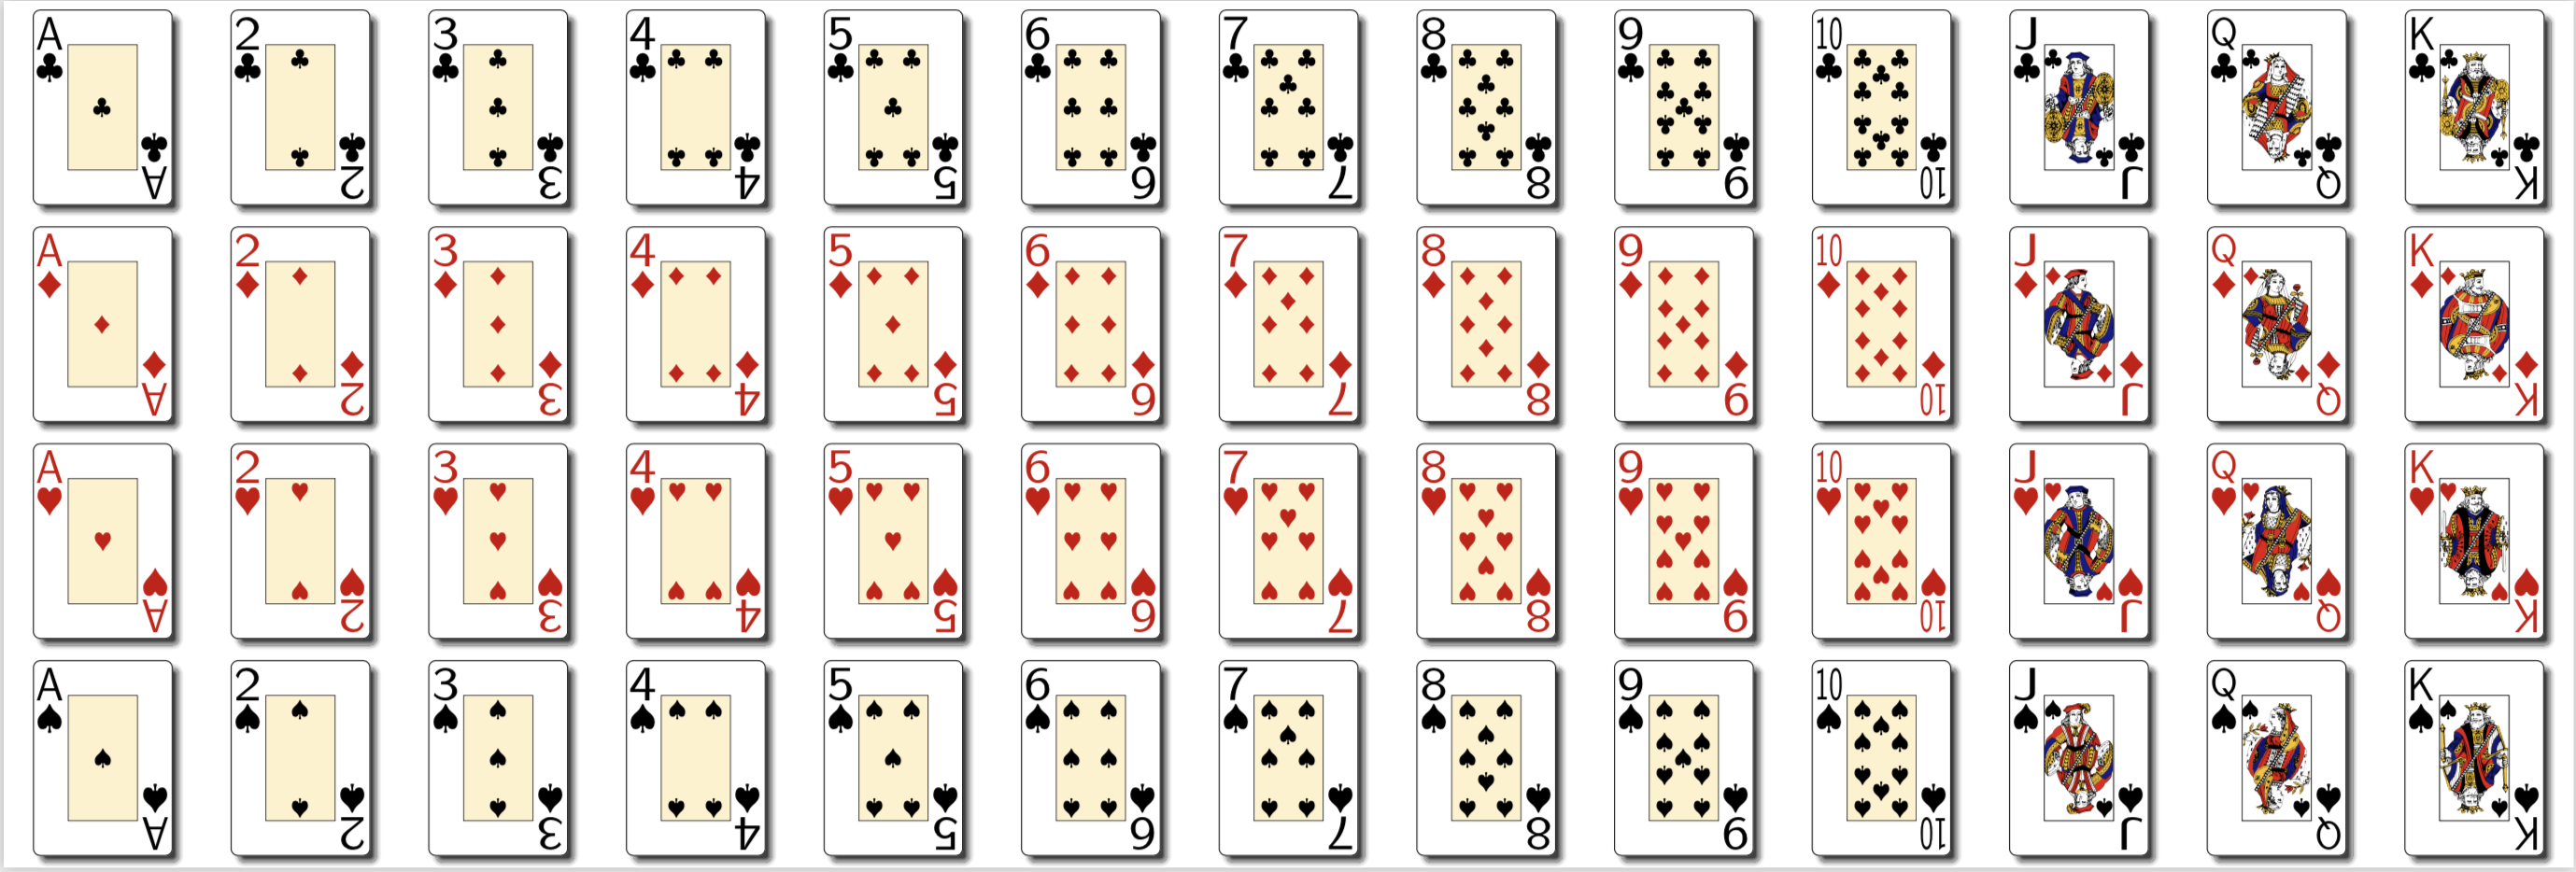
\includegraphics[scale=0.23]{../Images/Playing_Cards.png}
\end{center}
\end{frame}

\begin{frame}{Probability}
\begin{tcolorbox}[colframe=green!20!black, colback = green!30!white,title=\textbf{Probability}]
\textbf{Probability} is a measure of the likelihood of an event occurring.
\end{tcolorbox}
\vspace{6pt} \pause
\begin{center}
Probability = $\dfrac{\text{number of ways the event can occur}}{\text{total outcomes in sample space}}$
\end{center}
\end{frame}

\begin{frame}{Example 1}
Determine the probability of each event.	\newline\\
(a)	\quad	Flipping a coin and landing on heads \newline\\	\pause
1 outcome: Tails	\quad \pause 2 outcomes in sample space \pause
\[P(\text{heads}) = \frac{1}{2}\]
\end{frame}

\begin{frame}{Example 1}
(b)	\quad Rolling a number less than 3 on a single die.	\newline\\	\pause
2 outcomes: 1, 2	\quad	\pause	6 outcomes in sample space \pause
\[P(\text{rolling less than 3 on a single die}) = \frac{2}{6} = \frac{1}{3} \]
\end{frame}

\begin{frame}{Example 1}
(c)	\quad	Drawing a face card from a standard deck.	\newline\\	\pause
Face cards include jacks, queens, and kings. \newline\\	\pause
There are four suits for each card: clubs, diamonds, hearts, and spades.	\newline\\	\pause
Thus, there are 12 total face cards: jack of clubs, jack of diamonds, $\dots$, king of spades	\quad \pause There are 52 total cards	\pause
\begin{align*}
P(\text{drawing a face card}) &= \frac{12}{52} \\[6pt]	
P(\text{drawing a face card}) &= \frac{3}{13}
\end{align*}
\end{frame}

\end{document}